\chapter{Background}
\label{chap:background}
\lhead{\emph{Background}}

\section{Thematic Area within Computer Science}

The project of developing NoteReader, lies at the intersection of educational technology (EdTech) and software development. EdTech is a rapidly evolving field characterized by the integration of modern technologies into learning environments to enhance educational outcomes. Current trends in EdTech include the use of AI-driven personalized learning systems, immersive experiences through AR/VR, and data-driven analytics for adaptive learning paths.

However, unlike many modern EdTech initiatives that prioritize AI or AR/VR enhancements, this project addresses a more fundamental aspect of learning, the effective organization and access of study materials. By tackling the challenge of document-linked note-taking, NoteReader aims to simplify the learning process, reduce cognitive load, and enable efficient study workflows. Foundational learning strategies are essential, even as new technologies emerge.

To achieve its goals, this project draws upon principles from several key areas of computer science. These areas provide the theoretical and practical foundations required to develop a robust, scalable, and user-friendly application.

\section*{ACM Computing Classification System (CCS) Concepts}

\noindent
\textbf{Human-centered computing:} User interface design\\
\textbf{Information systems:} Document collection models\\
\textbf{Information systems:} Search interfaces\\
\textbf{Software and its engineering:} Software creation and management


 \section{A Review of Currently Available Alternatives}
This section reviews existing note-taking and document reading solutions to identify gaps in the market that NoteReader aims to fill. Key gaps include the lack of seamless integration between document viewing and note-taking, insufficient support for a wide range of document formats, limited cross-platform compatibility, and reliance on costly subscription-based cloud syncing services. 

Addressing these issues, NoteReader aims to provide a unified, subscription-free, and cross-platform solution that enables document-linked notes, multi-format support, and intuitive cataloging and search capabilities. The insights provided here will support the rationale for developing NoteReader and highlight the need for an integrated solution.

\subsection{Existing Note Taking Solutions}
    The findings below are based on my research into the feature availability of several note taking applications. This information is documented in an excel sheet. See attached file Existing Solutions Spreadsheet: \attachfile{existing_solutions.xlsx}. 
    
    A small excerpt of this file can be found in figure~\ref{fig:CD}.

    \begin{figure}
    \centering
    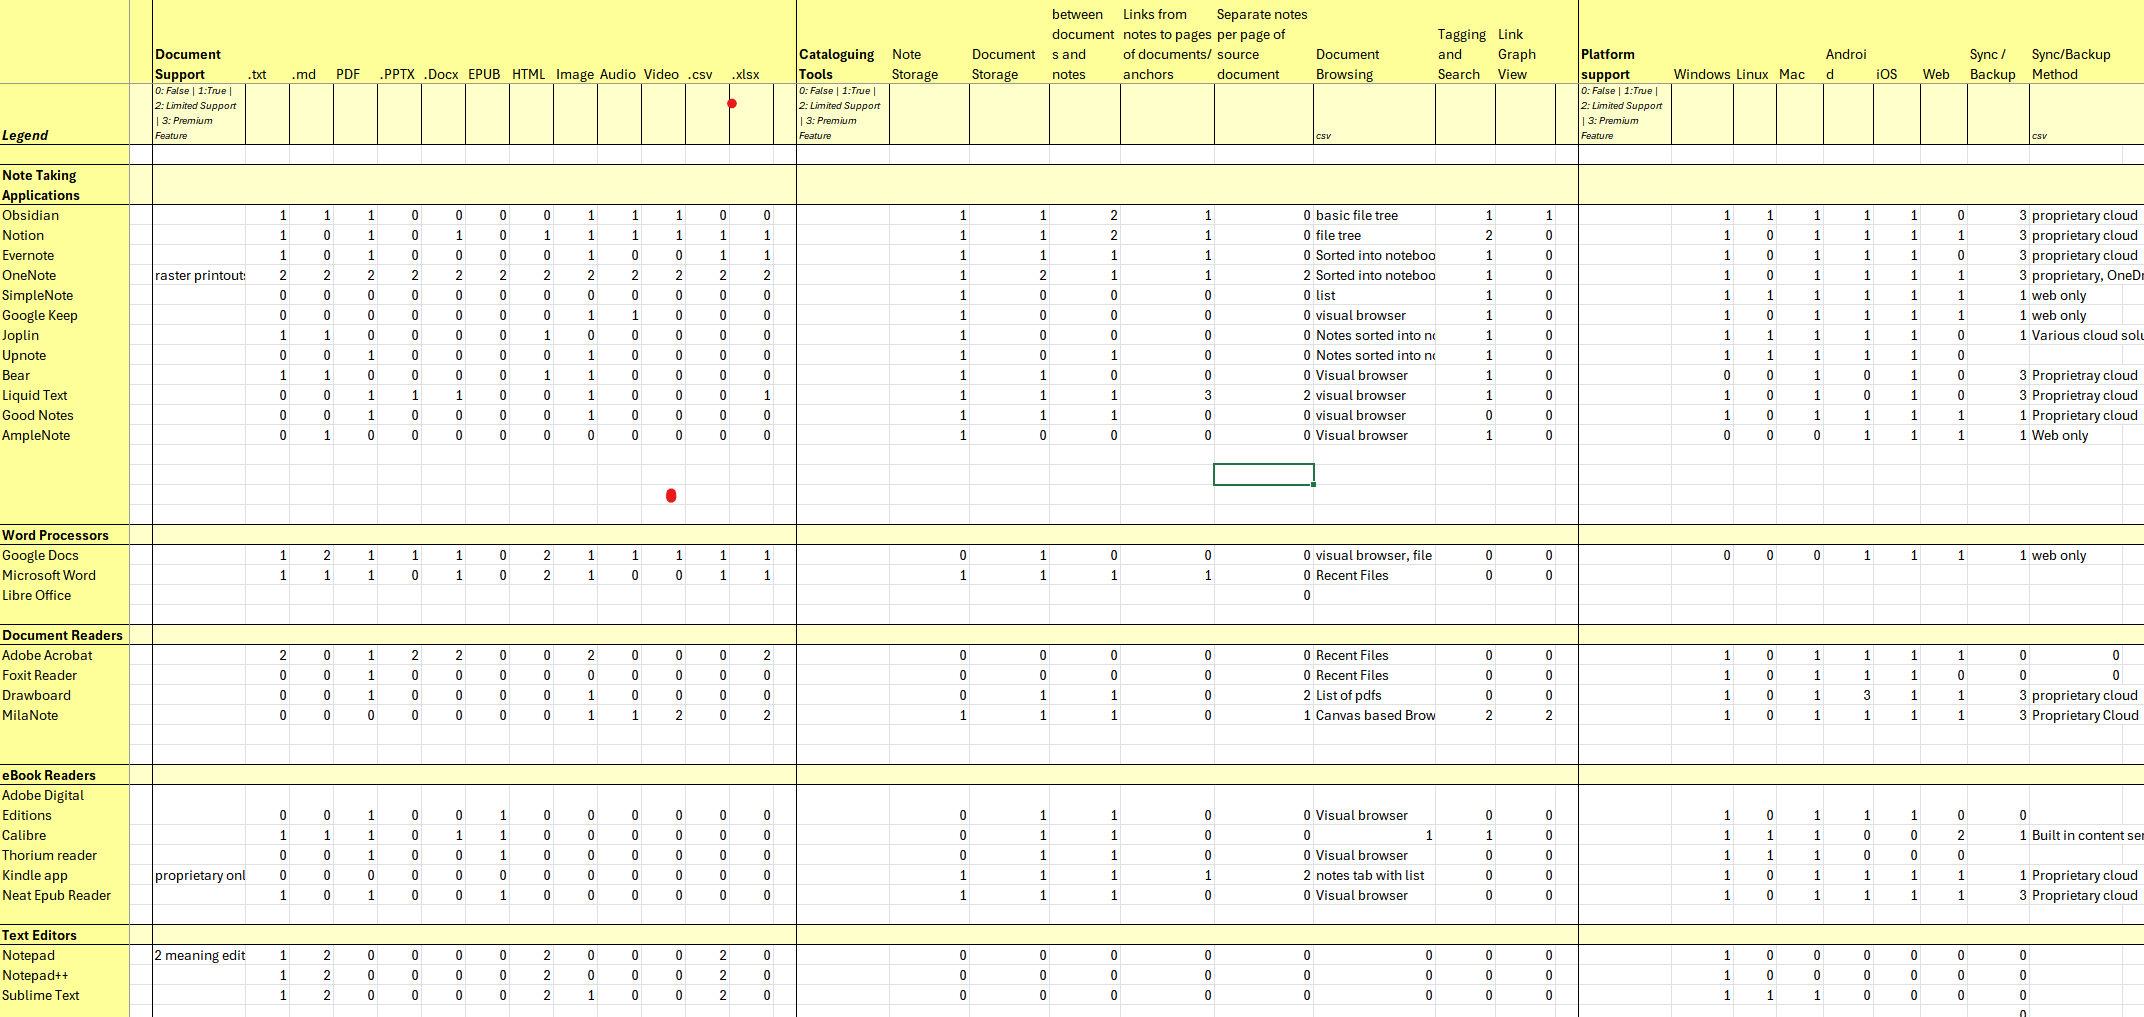
\includegraphics[width=1\linewidth]{Figures/existing solutions excerpt.png}
    \caption{Excerpt from the Existing Solutions Excel File, displaying some key findings (including document file-type support, cataloguing options and platform support)}
    \label{fig:Existing}
    \end{figure}

    \begin{figure}
        \centering
        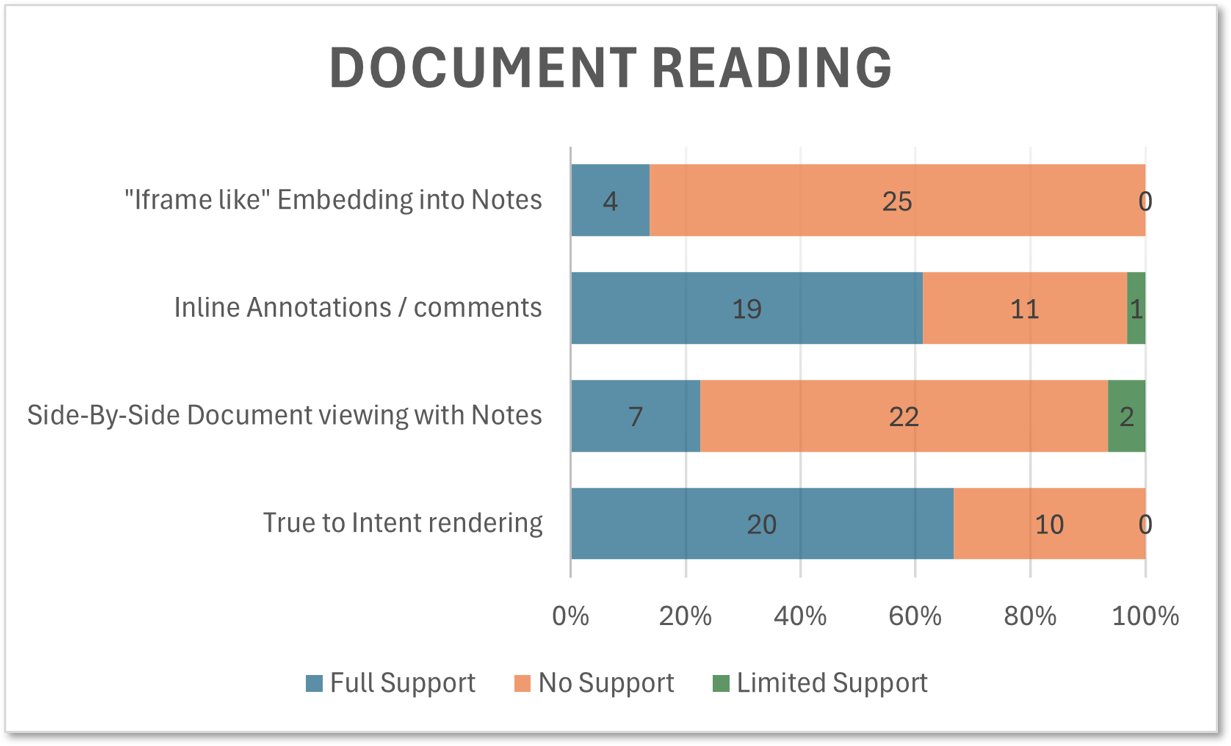
\includegraphics[width=1\linewidth]{Figures/docreading.png}
        \caption{Graph illustrating the support across reviewed applications for features including "True to Intent Rendering" and "Side by Side Viewing"}
        \label{fig:enter-label}
    \end{figure}
    \begin{figure}
        \centering
        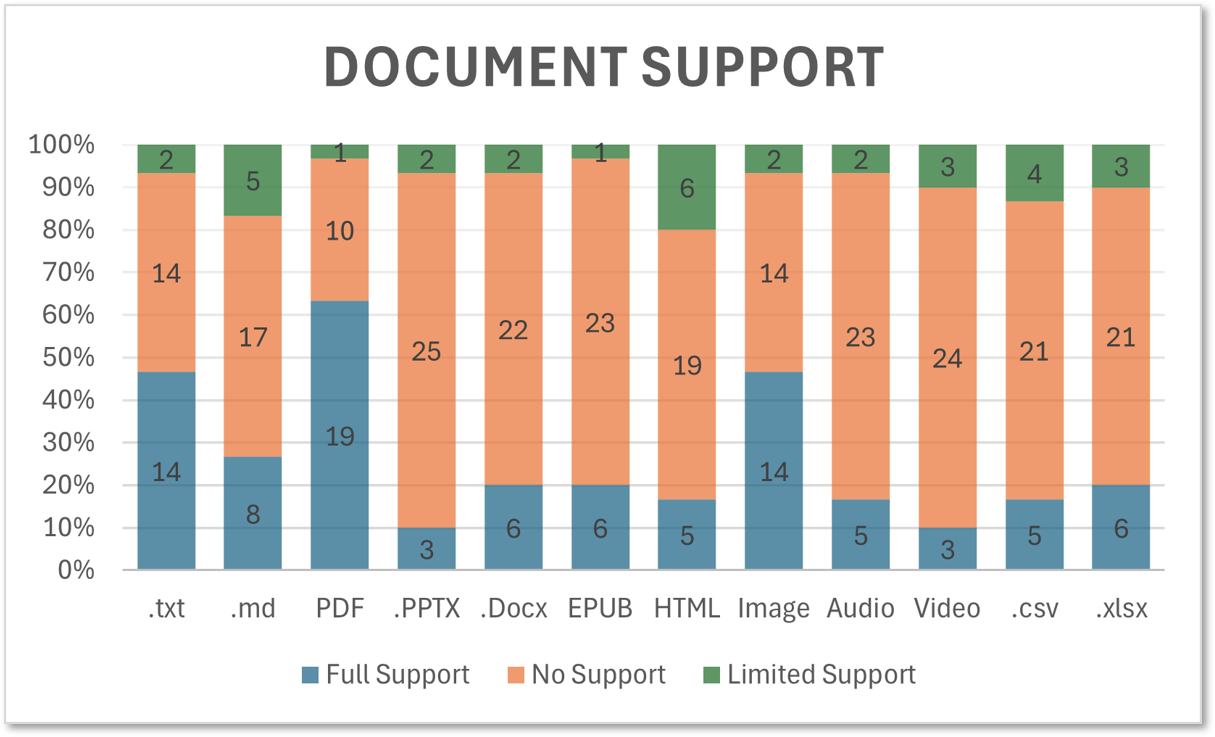
\includegraphics[width=1\linewidth]{Figures/docsupp.png}
        \caption{Graph illustrating the support across reviewed applications for document format}
        \label{fig:enter-label}
    \end{figure}
    \begin{figure}
        \centering
        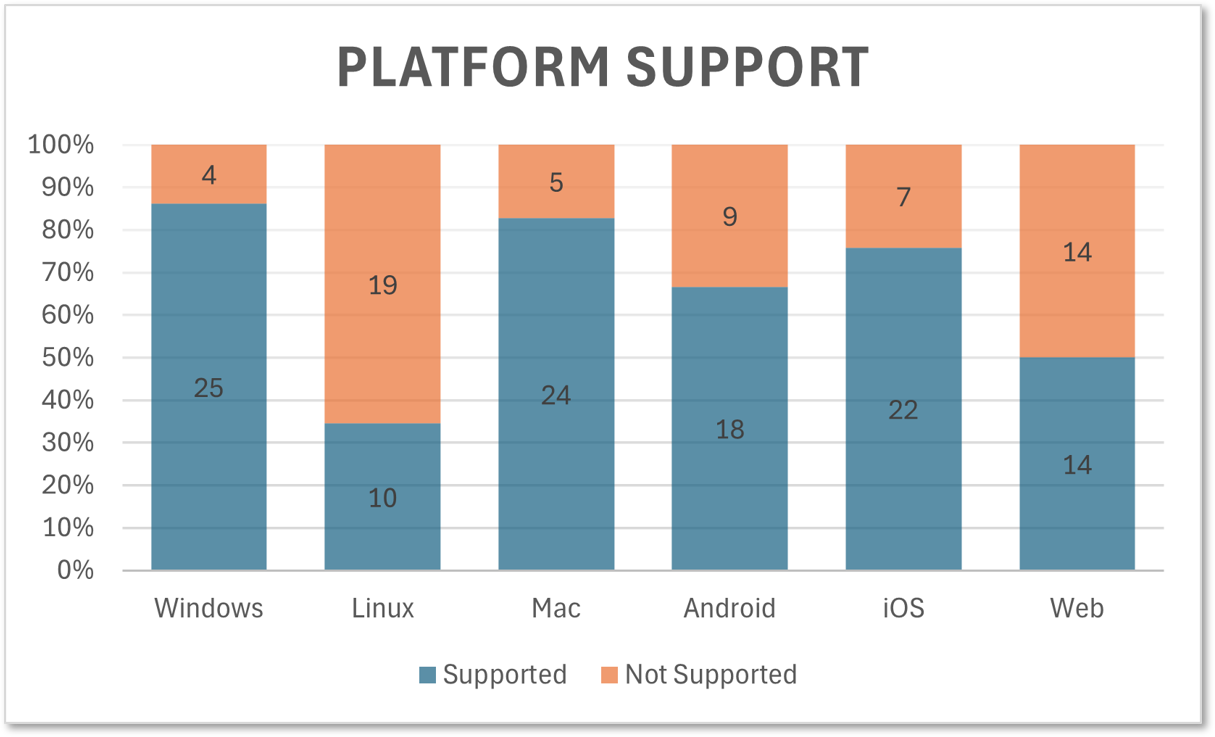
\includegraphics[width=1\linewidth]{Figures/platsupp.png}
        \caption{Graph illustrating the support across review applications for different platforms}
        \label{fig:enter-label}
    \end{figure}
    
	\begin{enumerate}
	    \item \textbf{Document file type support.} \\
        Very few applications support a wide range of common document types, and those which do do so using destructive methods, like raster printing of the document to a canvas, without storing the original. 
        
	    \item \textbf{File Syncing} \\
        Most note taking applications require a proprietary cloud service to sync between devices, or back up files. \\
        Version Control with remote repositories are not commonly used as a method of syncing this data.
    
	    \item \textbf{Dual functionality } \\
        Most document readers only allow notes via annotations, while most note taking applications only support document reading as embedded files. \\ 
        The ability to have side by side note taking and document reading is uncommon.
        
	    \item \textbf{Page of Notes per Page of Document} \\
        No application fully supports having linked notes with a separate page of notes per page of source document. Those which do support a similar function do so by adding all notes and pages to a large canvas for example Microsoft One Note. 
        
	    \item \textbf{Platform support.} \\
        Most applications tend to support only a couple of platforms. Linux support is especially rare for multiplatform applications.  
        
	    \item \textbf{Cost} \\
        Most note taking applications require some form of monthly subscription to use to their full potential. The pricing varies widely, as do the features on offer.
        
	\end{enumerate}

 \section{A Review of literature available on the effectiveness of digital note taking}

    In this section, I will review available literature on studies performed on the effectiveness of digital note taking, when compared to handwritten notes. 
    
    This review aims to better understand the benefits of the digital note-taking process to inform the development of NoteReader's user experience. The literature provides insight into the cognitive, procedural, and organizational aspects of digital note-taking, helping shape the design of the tool to meet the needs of learners.
 
    
    \subsection{Note-taking and Handouts in The Digital Age\cite{stacy_note_taking_2015}}

    In this article, the author explores the role of Handouts in lectures as a supplemental tool. The author discusses a number of challenges regarding handouts, pointing out that detailed handouts may lead to students not engaging in lectures, and simply memorizing the power point slides. They also suggest that a complete lack of handouts may result in students transcribing the full lecture material, rather than engaging in real time. 

    A compromise is suggested, where "skeletal" notes will provide a "scaffolding". This method gives a structure to note taking, without providing all information in the handouts themselves. The conclusion the author reaches here is that the student would be required to engage with the material, but not need to fully transcribe, just fill in the gaps. 

    This philosophy aligns well with the intended purpose and functionality of NoteReader. Source material acting as a scaffolding for personal notes, would be well supported by an application where pages of notes are displayed alongside pages of source material.

    By offering a side-by-side view, NoteReader facilitates a structure where students can engage deeply with the material without the cognitive overload of transcription.
    
    \subsection{Effectiveness of Digital Note-Taking on Students’ Performance in Declarative, Procedural and Conditional Knowledge Learning\cite{Sun2019}}
    
    This article describes a small trial of 72 Students, 40 taking digital notes, and 32 taking conventional handwritten notes. The author refers to three forms of knowledge Declarative, Procedural and Conditional, to differentiate between understanding of factual information, understanding of processes, and understanding of when to apply knowledge. Each will be measured separately in their study, and based on performance students are divided into percentiles. Notably this study focused on Computer Science students, in programming only. 

    Excellent students (those in the 70th percentile) showed improvement in all three knowledge types, but especially in declarative knowledge when using digital notes. Students below the 30th Percentile showed significant improvement in Conditional knowledge. Mid level students did not show significant improvement. 

    No group showed a decrease in performance when using digital notes. While this is a relatively small study, there is a suggestion that the advantages of digital note taking may be at least as effective as traditional methods. 

    The additional features proposed by NoteReader may be beneficial in further improving the performance difference of students taking digital notes. The split view link between source material and notes will allow students to study with improved context which may improve conditional understanding, when compared to memorization. This structured support mirrors the scaffolding identified as effective in the previous study\cite{stacy_note_taking_2015}.

    \subsection{Taking notes in the digital age: Evidence from classroom random control trials\cite{Artz2020}}
    
    This article describes a study to compare the effectiveness of digital note-taking compared to handwritten notes. 

    Some key findings were that exam scores showed no statistically significant difference between digital and handwritten notes. 
    
    There was however evidence that in subjects with high dependence on graphical or mathematical elements digital note taking may be at a disadvantage. Digital methods of creating diagrams, or mathematical equations tend to be more difficult and slower. 

    While not in scope for the initial round of development of NoteReader, inclusion of handwriting support and OCR may be a valuable addition to compensate for these weaknesses in a future release. 